\documentclass[12pt]{report}
\usepackage[utf8]{inputenc}
\usepackage[russian]{babel}
%\usepackage[14pt]{extsizes}
\usepackage{listings}

% Для листинга кода:
\lstset{ %
language=haskell,                 % выбор языка для подсветки (здесь это С)
basicstyle=\small\sffamily, % размер и начертание шрифта для подсветки кода
numbers=left,               % где поставить нумерацию строк (слева\справа)
numberstyle=\tiny,           % размер шрифта для номеров строк
stepnumber=1,                   % размер шага между двумя номерами строк
numbersep=5pt,                % как далеко отстоят номера строк от подсвечиваемого кода
showspaces=false,            % показывать или нет пробелы специальными отступами
showstringspaces=false,      % показывать или нет пробелы в строках
showtabs=false,             % показывать или нет табуляцию в строках
frame=single,              % рисовать рамку вокруг кода
tabsize=2,                 % размер табуляции по умолчанию равен 2 пробелам
captionpos=t,              % позиция заголовка вверху [t] или внизу [b] 
breaklines=true,           % автоматически переносить строки (да\нет)
breakatwhitespace=false, % переносить строки только если есть пробел
escapeinside={\#*}{*)}   % если нужно добавить комментарии в коде
}

% Для измененных титулов глав:
\usepackage{titlesec, blindtext, color} % подключаем нужные пакеты
\definecolor{gray75}{gray}{0.75} % определяем цвет
\newcommand{\hsp}{\hspace{20pt}} % длина линии в 20pt
% titleformat определяет стиль
\titleformat{\chapter}[hang]{\Huge\bfseries}{\thechapter\hsp\textcolor{gray75}{|}\hsp}{0pt}{\Huge\bfseries}


% plot
\usepackage{pgfplots}
\usepackage{filecontents}
\usetikzlibrary{datavisualization}
\usetikzlibrary{datavisualization.formats.functions}
\begin{filecontents}{levMtr.dat}
3 0.00003
4 0.00004
5 0.00005
6 0.00012 
7 0.00012
8 0.00016
9 0.00020
\end{filecontents}

\begin{filecontents}{levMtrTwo.dat}
3 0.00003
4 0.00004
5 0.00005
6 0.00012 
7 0.00012
8 0.00016
9 0.00020
12 0.00041
15 0.00058
\end{filecontents}

\begin{filecontents}{DamLevR.dat}
3 0.00003
4 0.0001
5 0.0008
6 0.004
7 0.02083
8 0.10250
9 0.57036
\end{filecontents}

\begin{filecontents}{DamLevT.dat}
3 0.00003
4 0.00004
5 0.00006
6 0.00008 
7 0.00012
8 0.00020
9 0.00025
\end{filecontents}

\begin{filecontents}{DamLevTTwo.dat}
3 0.00003
4 0.00004
5 0.00006
6 0.00008 
7 0.00012
8 0.00020
9 0.00025
12 0.00033
15 0.00041
\end{filecontents}

\tikzstyle{decision} = [diamond, draw, fill=blue!20, 
    text width=4.5em, text badly centered, node distance=3cm, inner sep=0pt]
\tikzstyle{block} = [rectangle, draw, fill=blue!20, 
    text width=5em, text centered, rounded corners, minimum height=4em]
\tikzstyle{line} = [draw, -latex']
\tikzstyle{cloud} = [draw, ellipse,fill=red!20, node distance=3cm,
    minimum height=2em]


\begin{document}
%\def\chaptername{} % убирает "Глава"
\begin{titlepage}
	\centering
	{\scshape\LARGE МГТУ им. Баумана \par}
	\vspace{3cm}
	{\scshape\Large Лабораторная работа №1\par}
	\vspace{0.5cm}	
	{\scshape\Large По курсу: "Анализ алгоритмов"\par}
	\vspace{1.5cm}
	{\huge\bfseries Расстояние Левенштейна\par}
	\vspace{2cm}
	\Large Работу выполнила: Подвашецкий Дмитрий, ИУ7-54Б\par
	\vspace{0.5cm}
	\LargeПреподаватели:  Волкова Л.Л., Строганов Ю.В.\par

	\vfill
	\large \textit {Москва, 2019} \par
\end{titlepage}

\tableofcontents

\newpage
\chapter*{Введение}
\addcontentsline{toc}{chapter}{Введение}
\textbf{Расстояние Левенштейна} - минимальное количество операций вставки, удаления, замены, необходимых для превращения одной строки в другую.

Расстояние Левенштейна в основном применяется для:

\begin{enumerate}
	\item для нахождения объектов или записей в поисковых системах;
	\item в базах данных, при поиске с неполно-заданным или неточно заданным именем;
	\item для исправления ошибок при вводе текста;
	\item для исправления ошибок в результате автоматического распознавания отсканированного текста или речи;
\end{enumerate}

Целью данной лабораторной работы является изучение алгоритмов Левенштейна и Дамерау-Левенштейна. 

Задачами данной лабораторной являются:
\begin{enumerate}
  	\item изучение алгоритмов Левенштейна и Дамерау-Левенштейна нахождения расстояния между строками;
	\item получение практических навыков реализации указанных алгоритмов: двух алгоритмов в матричной версии и одного из алгоритмов в рекурсивной версии; 
	\item экспериментальное подтверждение различий во временнóй эффективности рекурсивной и
нерекурсивной реализаций выбранного алгоритма; 
	\item описание и обоснование полученных результатов в отчете о выполненной лабораторной
работе, выполненного как расчётно-пояснительная записка к работе. 
\end{enumerate}


\chapter{Аналитическая часть}
Задача по нахождению расстояния Левенштейна заключается в поиске минимального количества операций вставки, удаления, замены, необходимых для превращения одной строки в другую.
 
\textbf{Действия обозначаются так:} 
\begin{enumerate}
  	\item D — удаление,
	\item I  — вставка,
	\item R  — замена,
	\item M — совпадение.
\end{enumerate}

Пусть $S_{1}$ и $S_{2}$ — две строки (длиной M и N соответственно) над некоторым алфавитом, тогда расстояние Левенштейна можно подсчитать по следующей рекуррентной формуле:

\begin{displaymath}
D(i,j) = \left\{ \begin{array}{ll}
 0, & \textrm{$i = 0, j = 0$}\\
 i, & \textrm{$j = 0, i > 0$}\\
 j, & \textrm{$i = 0, j > 0$}\\
min(\\
D(i,j-1)+1,\\
D(i-1, j) +1, &\textrm{$j>0, i>0$}\\
D(i-1, j-1) + m(S_{1}[i], S_{2}[j])\\
),
  \end{array} \right.
\end{displaymath}

где $m(a,b)$ равна нулю, если $a=b$ и единице в противном случае; $min\{\,a,b,c\}$ возвращает наименьший из аргументов.

При вычислении расстояния Дамерау-Левенштейна добавляется еще одна операция - транспозиция, т.е. перестановка двух соседних элементов.

Расстояние Дамерау-Левенштейна вычисляется по следующей рекуррентной формуле:
\begin{displaymath}
D(i,j) = \left\{ \begin{array}{ll}
max(i, j)&\textrm {if min($i,j$) = 0}\\
min(\\
D(i,j-1)+1,\\
D(i-1, j) +1,\\
D(i-1, j-1) + m(S_{1}[i], S_{2}[j])\\
D(i-2, j-2) + 1, &\textrm{if $i,j>1$ and $a_{i} = b_{j-1},a_{i-1}=b_{j} $}\\
min(\\
D(i,j-1)+1,\\
D(i-1, j) +1, &\textrm {otherwise}\\
D(i-1, j-1) + m(S_{1}[i], S_{2}[j])\\
)
  \end{array} \right.
\end{displaymath}

\chapter{Конструкторская часть}
\textbf{Требования к вводу:}
\begin{enumerate}
	\item Запрос на работу в тестовом режиме
  	\item Две строки, строчные и заглавные буквы считаются различными
\end{enumerate}
\textbf{Требования к программе:}
\begin{enumerate}
  	\item Корректный ввод, корректный вывод, программа не должна аварийно завершаться
\end{enumerate}

\begin{center}
    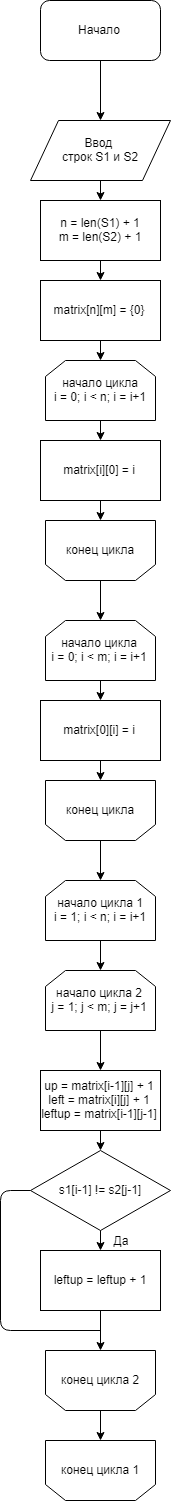
\includegraphics[scale=0.25]{lev_mtr}

    Схема 1. Матричный алгоритм Левенштейна
\end{center}

\begin{center}
    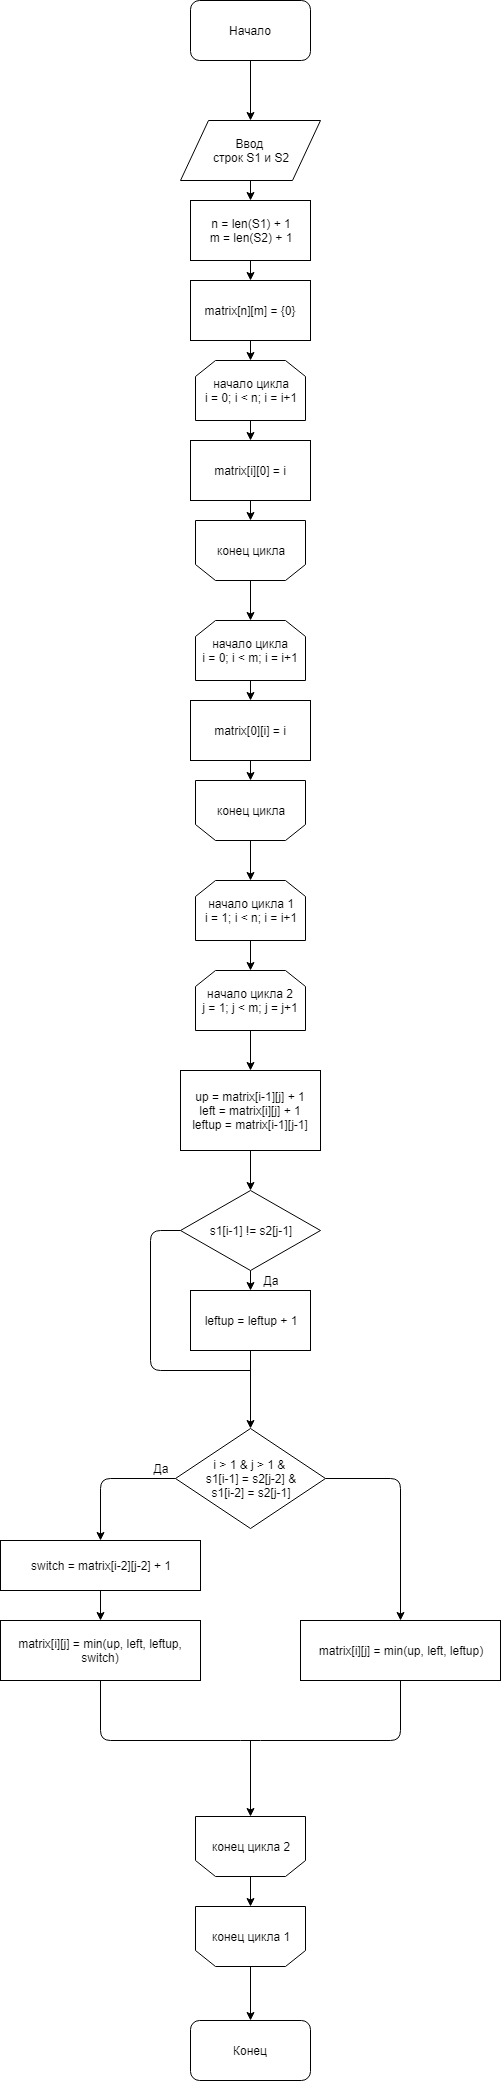
\includegraphics[scale=0.25]{dam_lev_mtr}

    Схема 2. Матричный алгоритм Дамерау-Левенштейна
\end{center}

\begin{center}
    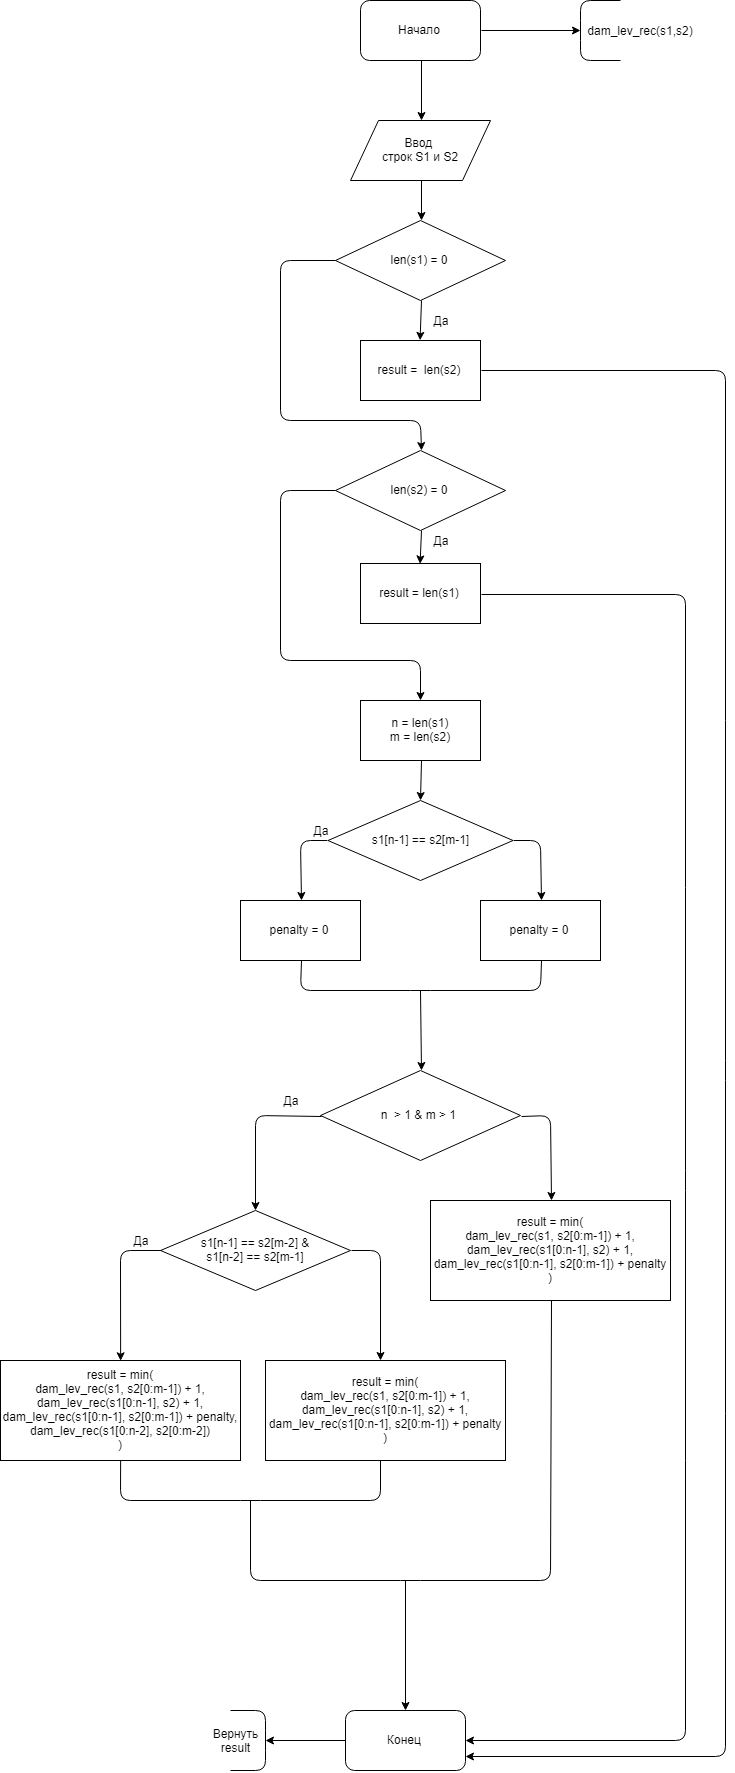
\includegraphics[scale=0.25]{dam_lev_rec}

    Схема 3. Рекурсивный алгоритм Дамерау-Левенштейна
\end{center}

\chapter{Технологическая часть}
\section{Выбор ЯП}
В качестве языка программирования был выбран Haskell, для ознакомления с ним.

\section{Замеры времени}
Замер времени работы алгоритмов производился при помощи функций getCurrentTime, diffUTCTime из библиотеки Data.Time.Clock.

Также производится усреднение времени работы улгоритмов. Для этого время считается для 12 вызовов, и после делится на 12.

\section{Сведения о модулях программы}
Программа состоит из:
\begin{itemize}
	\item main.hs - главный файл программы
	\item dam lev matrix.hs - файл с функцией вычисления расстояния Дамерау-Левенштейна матрично (Листинг 3.3)
	\item lev matrix.hs - файл с функцией вычисления расстояния Левенштейна матрично (Листинг 3.1)
	\item dam lev rec.hs - файл с функцией вычисления расстояния Дамерау-Левенштейна рекурсивно (Листинг 3.2)
	\item tests.hs - файл с тестами 
\end{itemize}

\begin{lstlisting}[label=some-code,caption=Функция нахождения расстояния Левенштейна матрично]
lev_mtr_abs :: String -> String -> Matrix Int
lev_mtr_abs s1 s2 = do
    let a = length s2
    let b = length s1
    let mtr = fromLists [[j | j <- [i..a+i]] | i <- [0..b]]
    
    lev_mtr s2 s1 2 2 mtr

cmp :: Char -> Char -> Int
cmp a b = if a == b
            then 0
            else 1

calc_min :: String -> String -> Int -> Int -> Matrix Int -> Int
calc_min s1 s2 i j mtr = minimum [(getElem (i-1) j mtr) + 1, 
                                  (getElem i (j-1) mtr) + 1,
                                  (getElem (i-1) (j-1) mtr) + (cmp (s1 !! (j-2)) (s2 !! (i-2)))]

                                
lev_mtr :: String -> String -> Int -> Int -> Matrix Int -> Matrix Int
lev_mtr "" s2 i j mtr = mtr
lev_mtr s1 "" i j mtr = mtr
lev_mtr s1 s2 i j mtr = 
    if i >= length s2 + 2
        then lev_mtr s1 s2 2 (j+1) mtr
        else if j >= length s1 + 2
            then mtr
            else lev_mtr s1 s2 (i+1) j (setElem (calc_min s1 s2 i j mtr) (i,j) mtr)
\end{lstlisting}

\begin{lstlisting}[label=some-code,caption=Функция нахождения расстояния Дамерау-Левенштейна рекурсивно]
cmp :: Char -> Char -> Int
cmp a b = if a == b
            then 0
            else 1

dam_lev_rec :: String -> String -> Int
dam_lev_rec "" s2 = length s2
dam_lev_rec s1 "" = length s1
dam_lev_rec s1 s2 = do
    let l1 = length s1
    let l2 = length s2
    if (l1 > 2) && (l2 > 2)
        then if ((last s1) == (s2 !! (l2-2)) && (s1 !! (l1-2)) == (last s2))
                then minimum [(dam_lev_rec (init s1)) s2 + 1, 
                              (dam_lev_rec s1 (init s2)) + 1,
                              (dam_lev_rec (init s1) (init s2)) + (cmp (last s1) (last s2)),
                              (dam_lev_rec (init (init s1)) (init (init s2))) + 1]
                              
                else minimum [(dam_lev_rec (init s1) s2) + 1, 
                              (dam_lev_rec s1 (init s2)) + 1,
                              (dam_lev_rec (init s1) (init s2)) + (cmp (last s1) (last s2))]
        else minimum [(dam_lev_rec "" s2) + 1, 
                      (dam_lev_rec s1 "") + 1,
                      (dam_lev_rec (init s1) (init s2)) + (cmp (last s1) (last s2))]
\end{lstlisting}

\begin{lstlisting}[label=some-code,caption=Функция нахождения расстояния Дамерау-Левенштейна матрично]
dam_lev_mtr_abs :: String -> String -> Matrix Int
dam_lev_mtr_abs s1 s2 = do
    let a = length s2
    let b = length s1
    let mtr = fromLists [[j | j <- [i..a+i]] | i <- [0..b]]
    
    dam_lev_mtr s2 s1 2 2 mtr

cmp :: Char -> Char -> Int
cmp a b = if a == b
            then 0
            else 1

calc_min :: String -> String -> Int -> Int -> Matrix Int -> Int
calc_min s1 s2 i j mtr = 
    if (i > 2) && (j > 2)
        then if ((s1 !! (j-2)) == (s2 !! (i-3))) && ((s1 !! (j-3)) == (s2 !! (i-2)))
            then minimum [(getElem (i-1) j mtr) + 1, 
                          (getElem i (j-1) mtr) + 1,
                          (getElem (i-1) (j-1) mtr) + (cmp (s1 !! (j-2)) (s2 !! (i-2))),
                          (getElem (i-2) (j-2) mtr) + 1]
                          
            else minimum [(getElem (i-1) j mtr) + 1, 
                          (getElem i (j-1) mtr) + 1,
                          (getElem (i-1) (j-1) mtr) + (cmp (s1 !! (j-2)) (s2 !! (i-2)))]
                          
        else minimum [(getElem (i-1) j mtr) + 1, 
                      (getElem i (j-1) mtr) + 1,
                      (getElem (i-1) (j-1) mtr) + (cmp (s1 !! (j-2)) (s2 !! (i-2)))]

dam_lev_mtr :: String -> String -> Int -> Int -> Matrix Int -> Matrix Int
dam_lev_mtr "" s2 i j mtr = mtr
dam_lev_mtr s1 "" i j mtr = mtr
dam_lev_mtr s1 s2 i j mtr = 
    if i >= length s2 + 2
        then dam_lev_mtr s1 s2 2 (j+1) mtr
        else if j >= length s1 + 2
            then mtr
            else dam_lev_mtr s1 s2 (i+1) j (setElem (calc_min s1 s2 i j mtr)  (i,j) mtr)
\end{lstlisting}

\chapter{Исследовательская часть}
Был проведен замер времени работы каждого из алгоритмов.

 
\begin{center}
Таблица. 1. Сравнение времени работы.   
	\begin{tabular}{|c c c c c|} 
 	\hline
	Длина (симв.) & dam lev rec (с) & lev mtr (с) & dam lev mtr (с) \\ [0.5ex] 
 	\hline\hline
 	3 &  0.00003 & 0.00003 & 0.00003\\
 	\hline
 	4 &  0.0001   & 0.00004 & 0.00004\\
 	\hline
	5 &  0.0008   & 0.00005 & 0.00006\\
	\hline
	6 &  0.04       & 0.00012 & 0.00008\\
	\hline
	7 &  0.02083 & 0.00012 & 0.00012\\
	\hline
	8 &  0.10250 & 0.00016 & 0.00020\\
	\hline
	9 &  0.57036 & 0.00020 & 0.00025\\
	\hline
	\end{tabular}
\end{center}




\begin{center}
\begin{tikzpicture}
\begin{axis}[
    	axis lines = left,
    	xlabel = $Len (symbols)$,
    	ylabel = $time (sec)$,
	legend pos=north west,
	ymajorgrids=true
]
\addplot[color=orange] table[x index=0, y index=1] {DamLevR.dat};
\addplot[color=blue, mark=square] table[x index=0, y index=1] {levMtr.dat};
\addplot[color=green, mark=square] table[x index=0, y index=1] {DamLevT.dat};

\addlegendentry{dam lev rec}
\addlegendentry{ lev mtr}
\addlegendentry{dam lev mtr}
\end{axis}
\end{tikzpicture}

Рис. 1. График вермени работы всех трех алгоритмов.
\end{center}

\begin{center}
\begin{tikzpicture}
\begin{axis}[
    	axis lines = left,
    	xlabel = $Len (symbols)$,
    	ylabel = $time (sec)$,
	legend pos=north west,
	ymajorgrids=true
]
\addplot[color=blue, mark=square] table[x index=0, y index=1] {levMtrTwo.dat};
\addplot[color=green, mark=square] table[x index=0, y index=1] {DamLevTTwo.dat};

\addlegendentry{lev mtr}
\addlegendentry{dam lev mtr}
\end{axis}
\end{tikzpicture}

Рис. 2. График вермени работы матричных алгоритмов.
\end{center}

\par
Матричные реализации практически не отличаются друг от друга по времени. В то время как рекурсивная уже при длине строк больше 5 работает медленее в десятки раз.

\chapter*{Заключение}
\addcontentsline{toc}{chapter}{Заключение}

Мною были изучены алгоритмы Левенштейна и Дамерау-Левенштейна нахождения расстояния между строками.

Также мною получены практические навыки раелизации указанных алгоритмовв матричной  и рекурсивных версиях. 

Экспериментально было проверено различие во временной эффективности рекурсивной и нерекурсивной реализаций алгоритма Дамерау-Левенштейна.

Было произведено описание и обоснование полученных результатов.

В результате можно сделать вывод, что практически всегда предпочтительнее использовать матричный вариант.

\end{document}